%\documentclass[12pt]{article}
\documentclass[12pt]{extarticle}
\usepackage[utf8]{inputenc}
\usepackage[margin=0.5in]{geometry}
\usepackage{enumitem}
\usepackage{graphicx}
\usepackage{float}
\usepackage{romannum}
\usepackage{xunicode}
 
 % Title page
\title{VAST 2019 Report 3}
\author{Vivek Koodli Udupa \\ Madhumita Krishnan}
\date{\today}

\begin{document}
\pagenumbering{arabic}
\maketitle

% INTRODUCTION
\begin{centering}
	\section{Introduction}
\end{centering}
This report addresses the issue of dealing with missing values in the given dataset. Does a missing value in a particular damage category say that the damage is zero or does it say that the person failed to record a value? Replacing all the missing value with zero could have adverse effects. \\

The process of replacing a missing value is termed as \textbf{Imputation}. Imputing missing values by zeros will bring the category average down by a considerable margin. One way to counter this issue is to impute the missing values by the category mean. \\

As established in the previous report, St. Himark was hit by a disastrous earthquake on April $8^{th}$, 2020 at 8am. The damage report contains reports coming in from various time ranges, including the ones before the earth quake. Does excluding these reports give a better idea of the effects of the earthquake and the extent of damage caused by the earthquake?  \\

This report visualizes the effects of mean imputation over zero imputation for the Mini Challenge 1 of the VAST 2019 dataset. This report will also visualize the damages caused before, during and after the earthquake to get a clear idea of the extent of damage sustained by St. Himark during this unfortunate event. \\


% \\
% As we spoke in our last report, we wanted to bring in time series and box plots to address data credibility.  \\
% Imputation was another issue. Missing values were replaced with zeros, does replacing them with mean of the damage type for each location make a difference? \\



% %Plot of Maps
% \begin{figure}[H]
% 	\centering
% 	\begin{minipage}{0.5\textwidth}
% 		\centering
% 		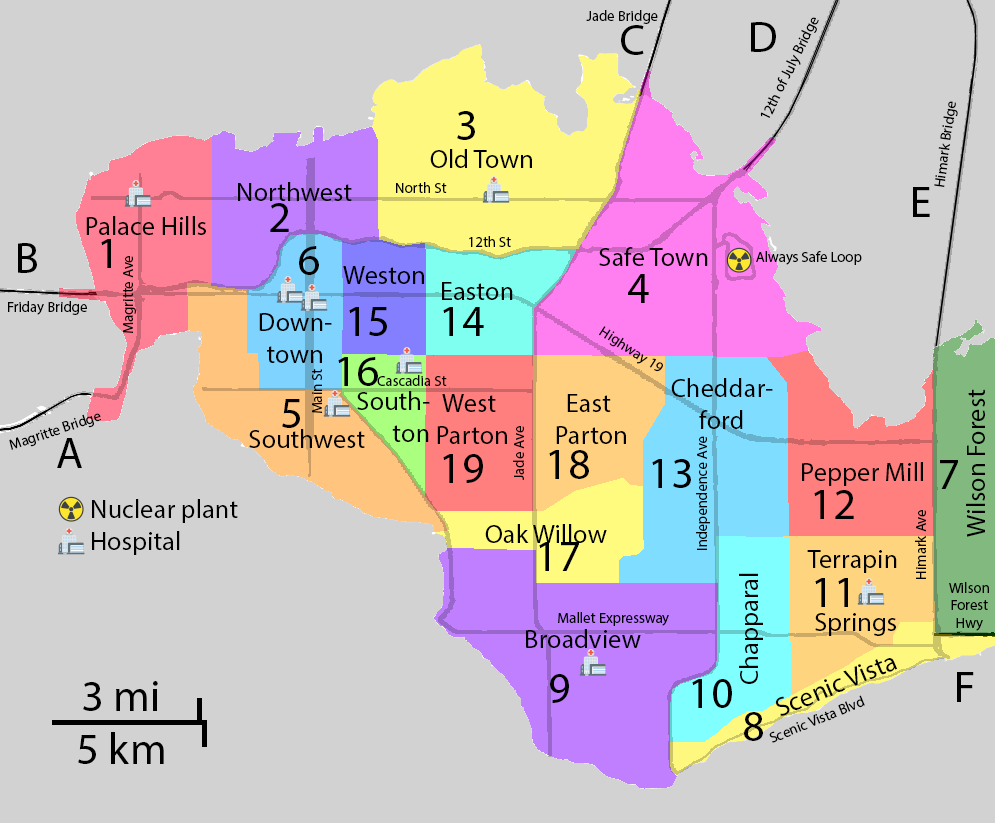
\includegraphics[width=\textwidth]{Images/map.png}
% 		\caption{St.Himark Neighborhood Map}
% 		\label{fig:map}
% 	\end{minipage}%
% 	\begin{minipage}{0.5\textwidth}
% 		\centering
% 		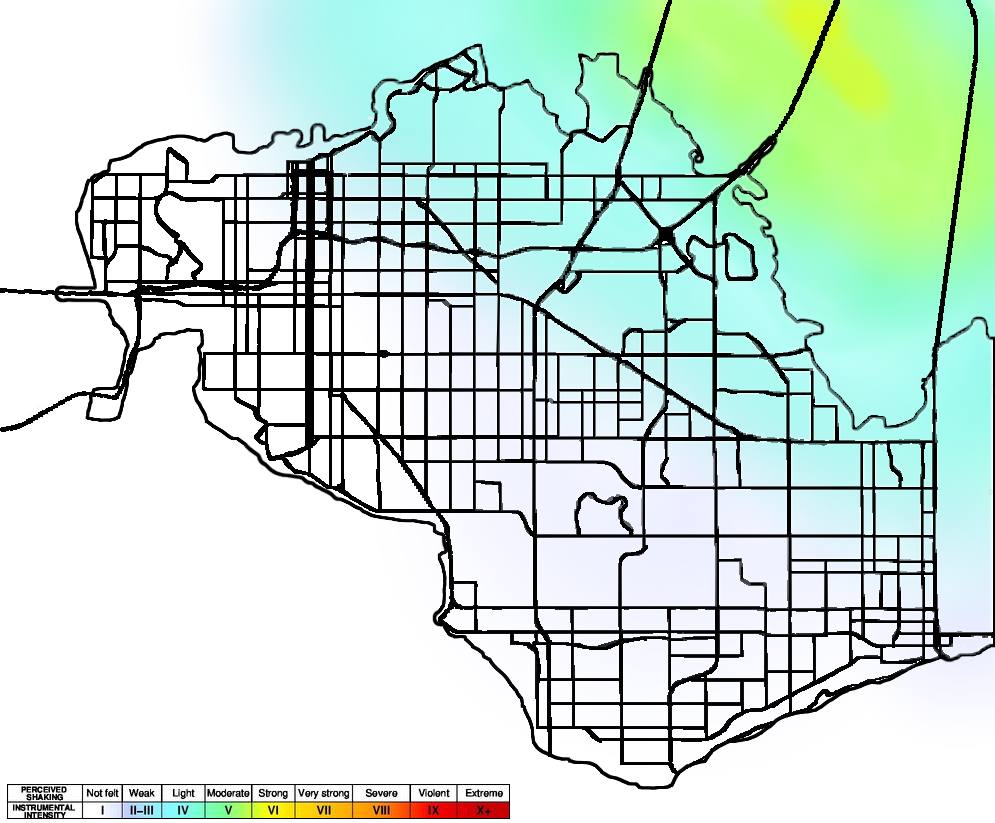
\includegraphics[width=\textwidth]{Images/shakemap.png}
% 		\caption{St.Himark Shake Map}
% 		\label{fig:shakemap}
% 	\end{minipage}
% \end{figure} 

% % Damage plot
% \begin{figure}[H]
% \centering
% 	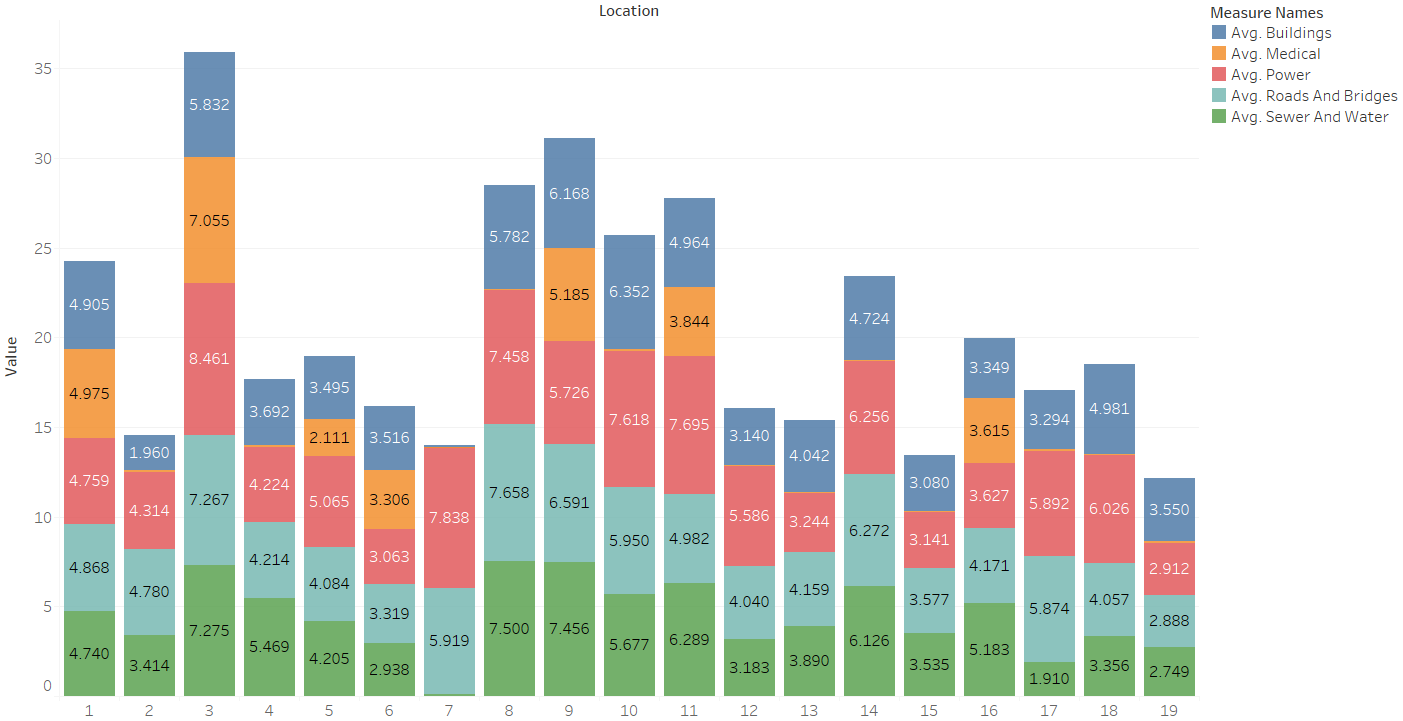
\includegraphics[width=\linewidth]{Images/AllDamage.png}
% 	\caption{Cumulative damage for different locations }
% 	\label{fig:alldamage}
% \end{figure}
%Analysis and Visualization
\begin{centering}
    \section{Analysis and Visualization}
\end{centering}
\subsection{Imputation}
The first change made to Data Pre-processing was replacing the missing values with the mean of damage values for each location. On completing this process the following plots were derived. \\

Figures \ref{fig:SIImp} through \ref{fig:PowerImp} shows the comparison between the damage reports imputed with zero's and respective damage category mean for individual locations. The Blue graph represents the mean imputed dataset and the orange graph represents the zero imputed dataset.\\

\begin{figure}[H]
	\centering
	\begin{minipage}{0.5\textwidth}
		\centering
		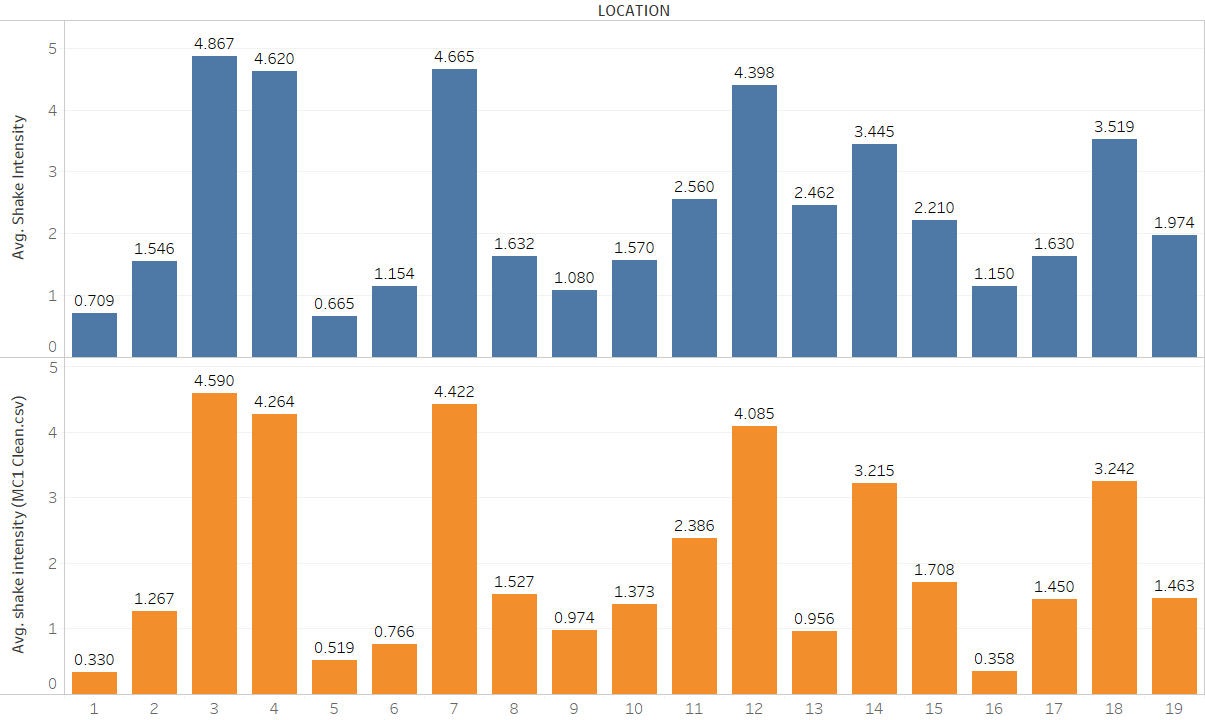
\includegraphics[width=\textwidth]{SIAvg.png}
		\caption{Shake Intensity Imputation}
		\label{fig:SIImp}
	\end{minipage}%
	\begin{minipage}{0.5\textwidth}
		\centering
		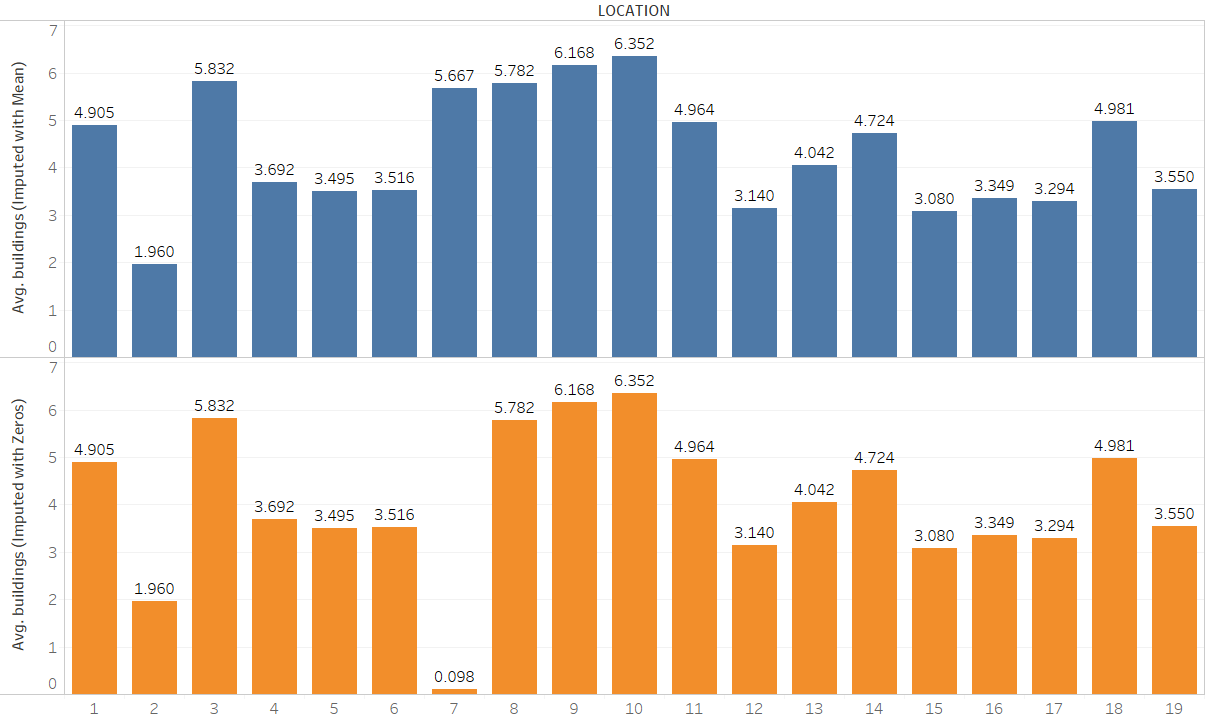
\includegraphics[width=\textwidth]{Building.png}
		\caption{Building damage Imputation}
		\label{fig:BuildingImp}
	\end{minipage}
\end{figure} 


\begin{figure}[H]
	\centering
	\begin{minipage}{0.5\textwidth}
		\centering
		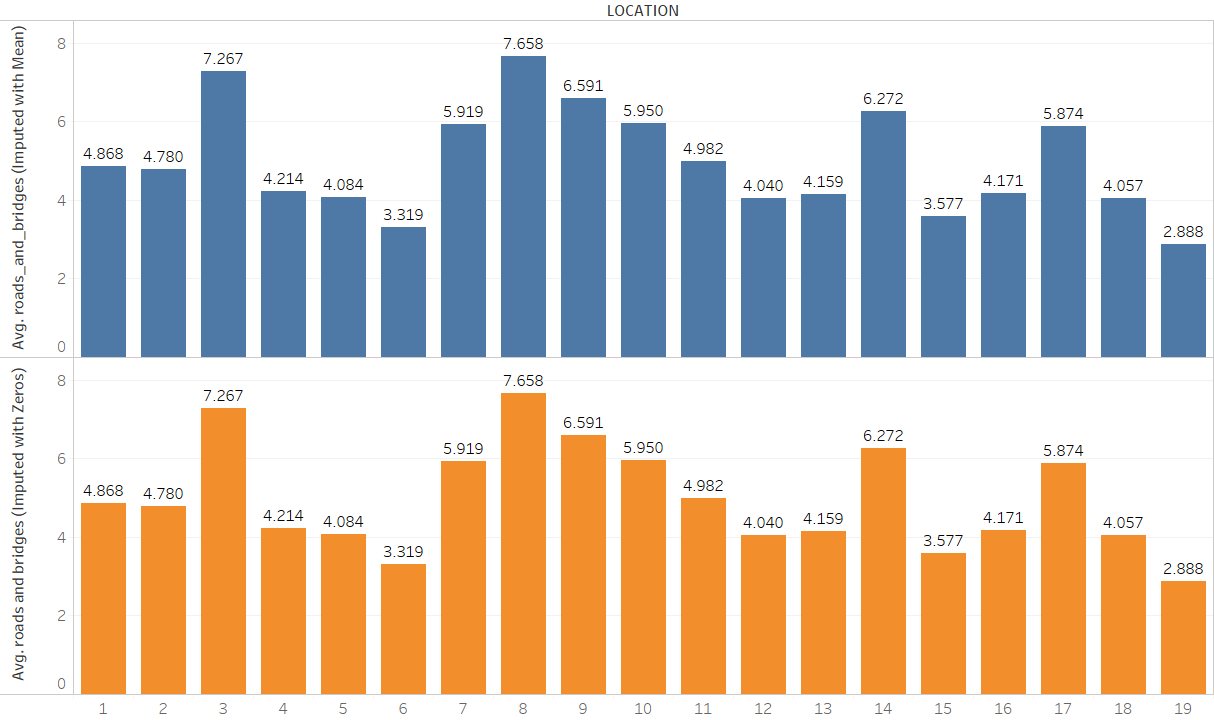
\includegraphics[width=\textwidth]{Road.png}
		\caption{Road damage Imputation}
		\label{fig:RoadImp}
	\end{minipage}%
	\begin{minipage}{0.5\textwidth}
		\centering
		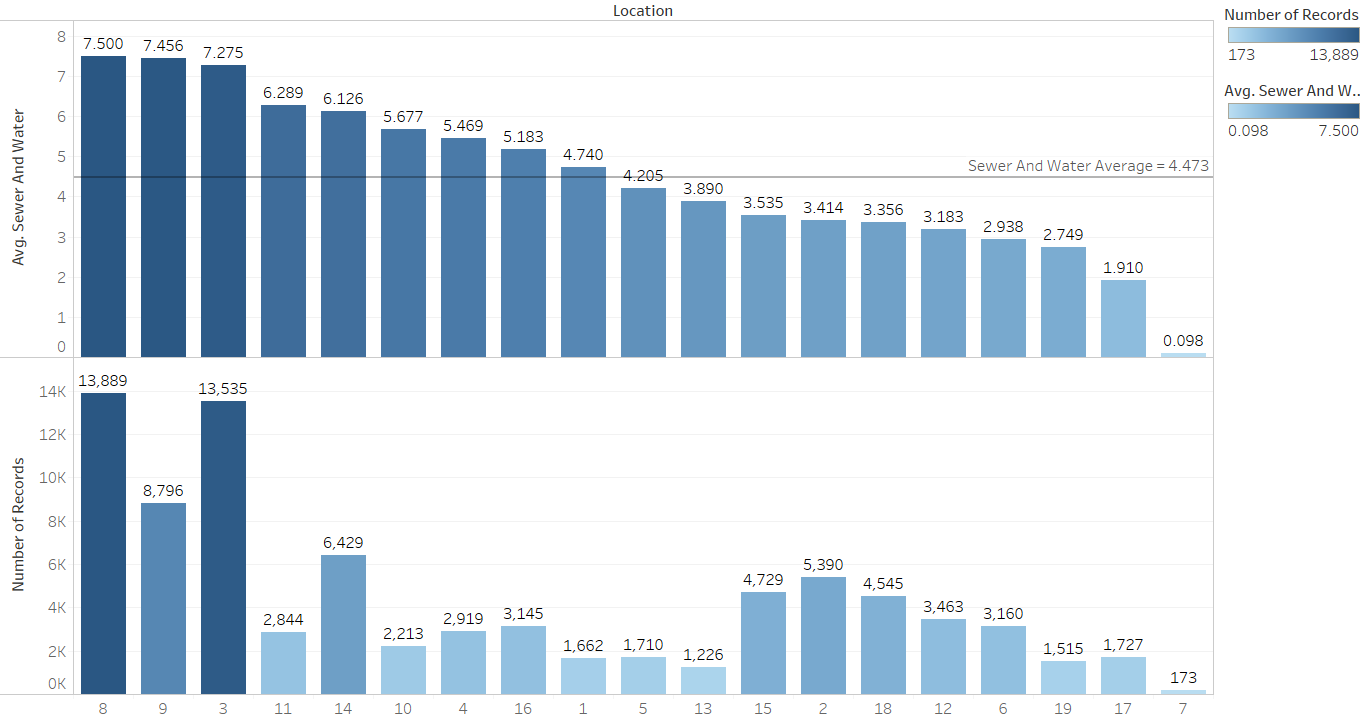
\includegraphics[width=\textwidth]{Water.png}
		\caption{Water damage Imputation}
		\label{fig:WaterImp}
	\end{minipage}
\end{figure} 


\begin{figure}[H]
	\centering
	\begin{minipage}{0.5\textwidth}
		\centering
		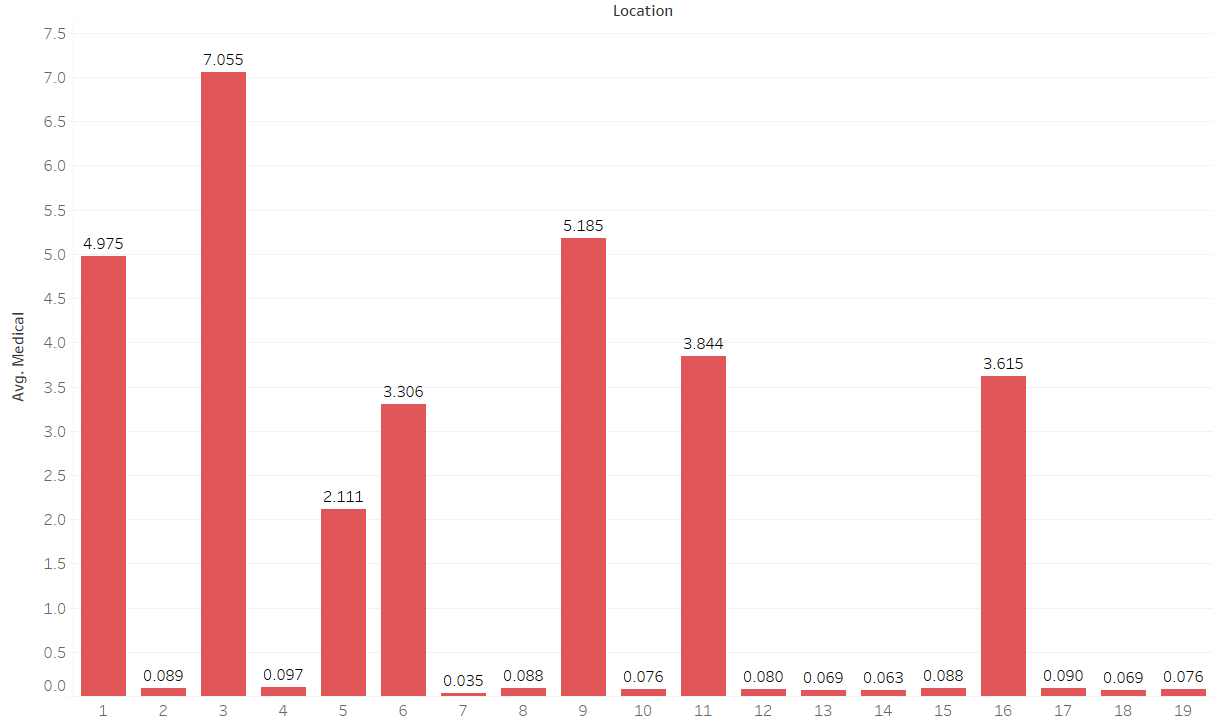
\includegraphics[width=\textwidth]{Medical.png}
		\caption{Medical damage Imputation}
		\label{fig:MedicalImp}
	\end{minipage}%
	\begin{minipage}{0.5\textwidth}
		\centering
		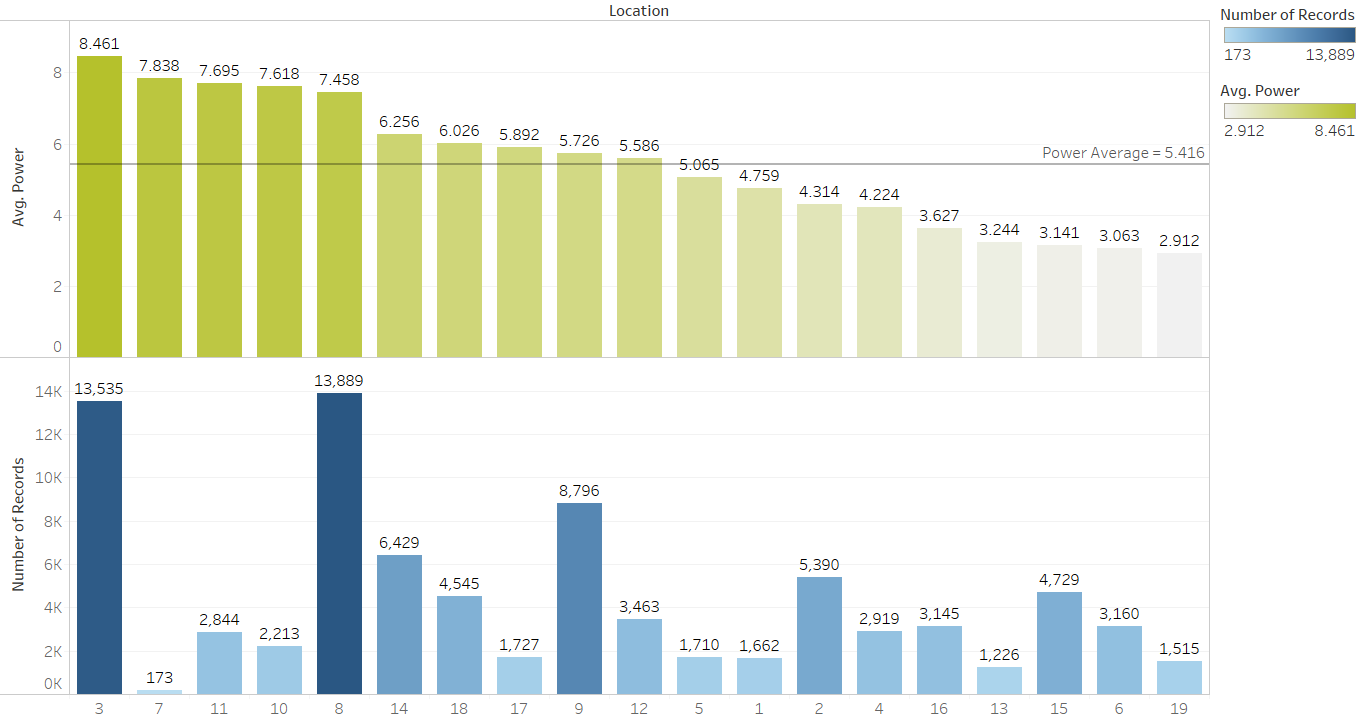
\includegraphics[width=\textwidth]{Power.png}
		\caption{Power damage Imputation}
		\label{fig:PowerImp}
	\end{minipage}
\end{figure} 

On analyzing Figure \ref{fig:MedicalImp}, it can be observed that the average Medical damage values with mean imputation shows a drastic increase for certain locations as compared to average Medical damages which were imputed with zeros. On further inspection it was noted that all the missing Medical damage reports corresponded to the locations where no hospitals were present. \\  

Figure \ref{fig:BuildingImp} and Figure \ref{fig:WaterImp} also show similar effects for location 7. The remaining Figures display similar patterns for mean and zero imputations.  \\

\subsection{Time-Series Analysis}
 This section of the report visualizes the damages recorded before, during and after the earthquake on April $8^{th}$, 2020. 

\begin{figure}[H]
\centering
	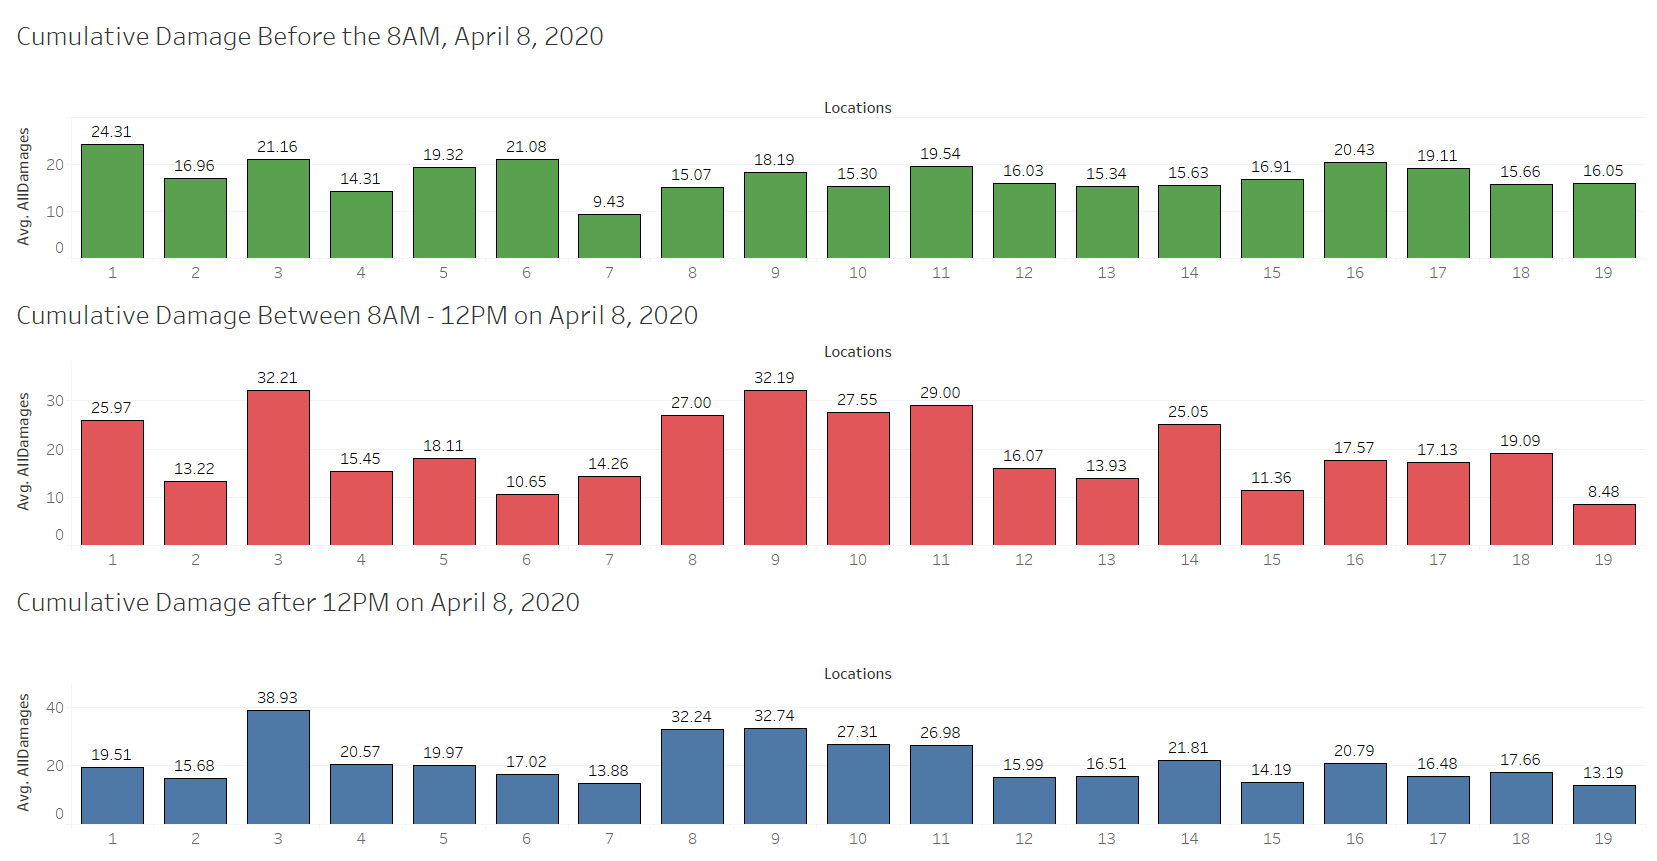
\includegraphics[width=\linewidth]{TSAllDamage.png}
	\caption{Average Cumulative Damage for different time instances }
	\label{fig:TSA}
\end{figure}

Figure \ref{fig:TSA} shows the average cumulative damage sustained by each location of St. Himark before, during and after the earthquake. Each bar represents the average of sum of 5 types of damages sustained by each location. \\

% Figure \ref{fig:TSA} represents the average cumulative damages for three different time frames. The green plot shows the damage for all time instances that have been recorded. The red plot displays the damage recorded after 8 am, which is the assumed instance of earth quake. The blue plot represents the damages recorded for a small time frame i.e, 8am to 12pm. \\

The purpose of Figure \ref{fig:TSA} was to visualize the importance of time instance at which the damage reports were recorded. The assumed time instance at which the earth quake hit St.Himark was 8am on \(8^{th}\) April 2020. This means that the reports received before 8am can be labelled as damages that were not caused by the earthquake and can be ignored for this analysis. A smaller time period, 8am - 12pm was explored in order to determine if the reports that came long after the earth quake affected the judgment of the people reporting the damage. The hypothesis is that the accuracy at which the people judged the damage immediately after the earthquake would be higher in comparison to that when done long after the earthquake. 
%Add the next image here
\begin{figure}[H]
\centering
	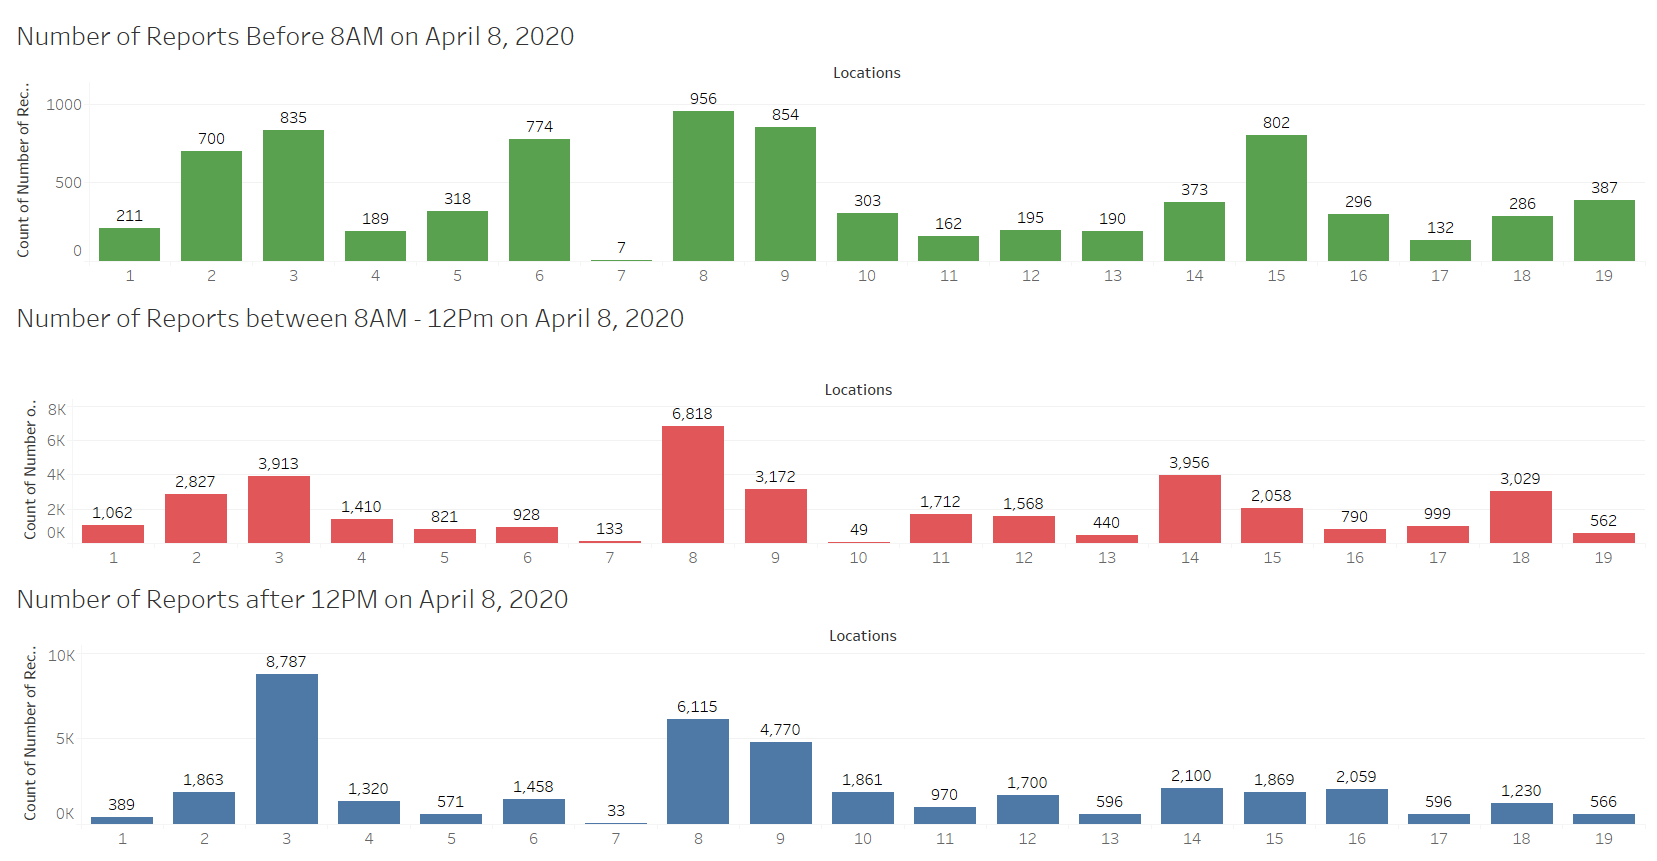
\includegraphics[width=\linewidth]{NumberOfReports.png}
	\caption{Number of Records for different time instances }
	\label{fig:TSS}
\end{figure}
 
 In figure \ref{fig:TSS} the uncertainty of the data using time series is analyzed. The green plot in the figure represents Number of Reports recorder before the assumed time of the earth quake i.e, 8 am. The red plot shows the Number of Reports between 8 am and 12 pm. Similarly the blue plot shows all the records after 12pm on \(8^{th}\) April. \\
 
 Since an assumption is made that the earth quake takes place between 8am-12pm any damage reports before this time frame can be ignored. From Figure \ref{fig:TSS}, it can be observed that there are 7970 reports before the earth quake, 36247 reports during the time frame of the earth quake and 38853 reports recorded after the assumed time period of the earth quake. Thus 7970 reports can be classified as damages not caused by the earth quake. \\ 
 
 Figure \ref{fig:SiTSA} shows the shake intensities recorded at different time instances. It can be observed that the shake intensities recorded before the earthquake is insignificant. The shake intensities during and after the earthquake shows similar pattern. \\
 
 %Shake Intensity TSA Plot
 \begin{figure}[H]
\centering
	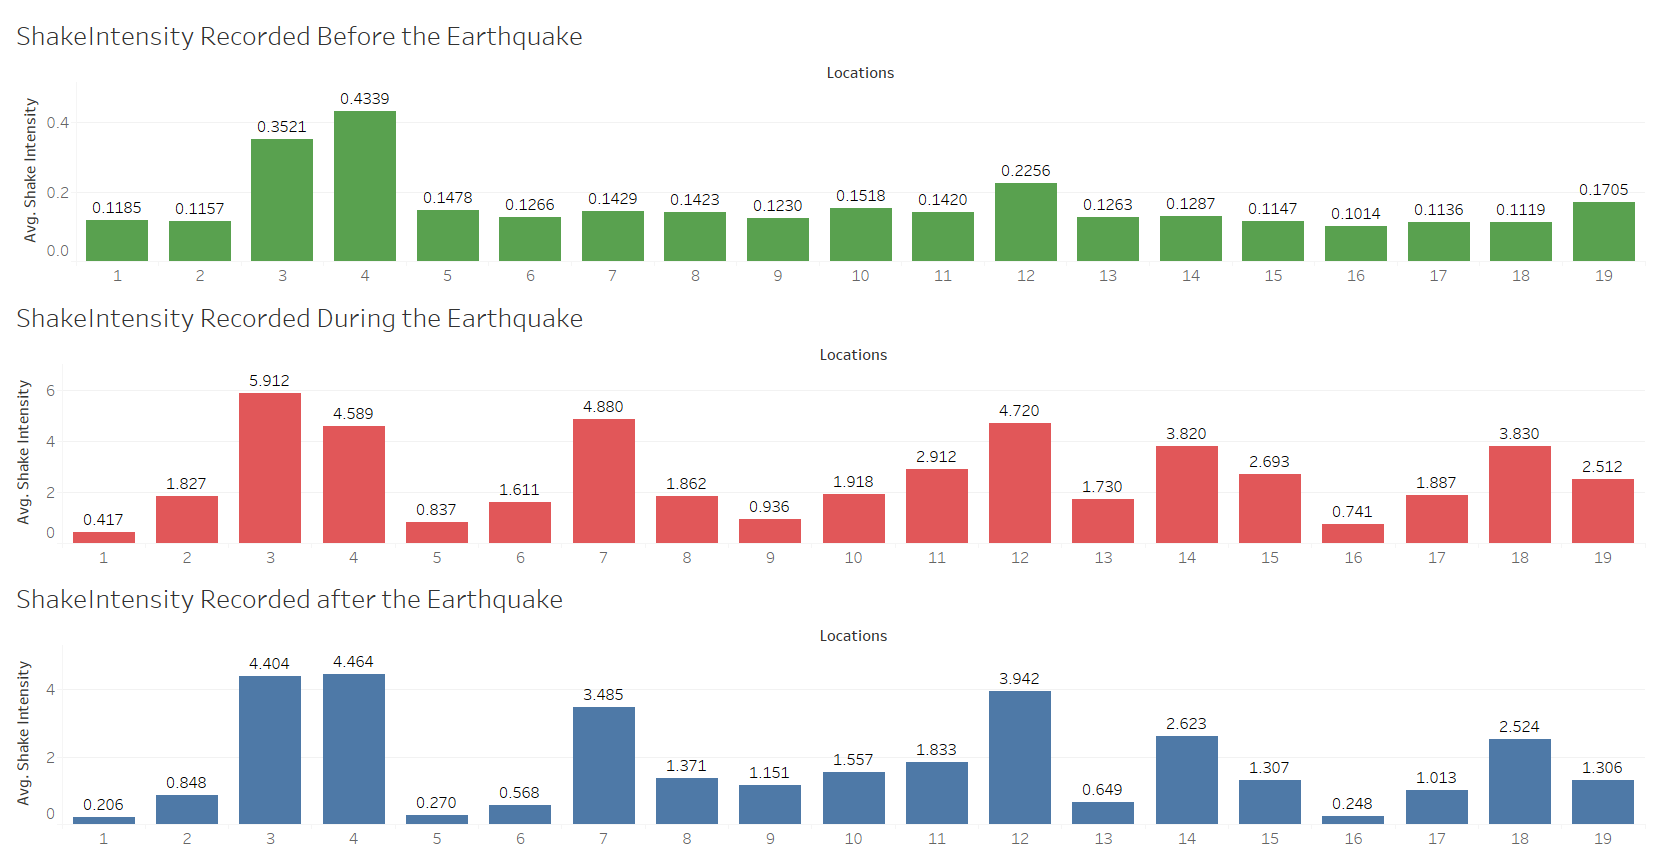
\includegraphics[width=\linewidth]{ShakeIntTSA.png}
	\caption{Shake Intensities Recorded at different time instances }
	\label{fig:SiTSA}
\end{figure}
 
%Box Plots
\subsection{Box Plots}

\begin{figure}[H]
	\centering
	\begin{minipage}{0.5\textwidth}
		\centering
		\includegraphics[width=\textwidth]{SIBoxPlt.png}
		\caption{Box Plot for Shake Intensity}
		\label{fig:SIBoxPlt}
	\end{minipage}%
	\begin{minipage}{0.5\textwidth}
		\centering
		\includegraphics[width=\textwidth]{BuildingsBoxPlt.png}
		\caption{Box Plot for Building damage}
		\label{fig:BuildingBoxPlt}
	\end{minipage}
\end{figure} 
\begin{figure}[H]
	\centering
	\begin{minipage}{0.5\textwidth}
		\centering
		\includegraphics[width=\textwidth]{RoadBoxPlt.png}
		\caption{Box Plot for Roads and Bridges damage}
		\label{fig:RoadBoxPlt}
	\end{minipage}%
	\begin{minipage}{0.5\textwidth}
		\centering
		\includegraphics[width=\textwidth]{SewerAndWaterBoxPlt.png}
		\caption{Box Plot for Sewer and Water damage}
		\label{fig:WaterBoxPlt}
	\end{minipage}
\end{figure} 
\begin{figure}[H]
	\centering
	\begin{minipage}{0.5\textwidth}
		\centering
		\includegraphics[width=\textwidth]{MedicalBoxPlt.png}
		\caption{Box Plot for Medical damage}
		\label{fig:MedicalBoxPlt}
	\end{minipage}%
	\begin{minipage}{0.5\textwidth}
		\centering
		\includegraphics[width=\textwidth]{PowerBoxPlt.png}
		\caption{Box Plot for Power damage}
		\label{fig:PowerBoxPlt}
	\end{minipage}
\end{figure} 

%Conclusion
\begin{centering}
	\section{Conclusion}
\end{centering}
This report tried to address the issues of missing values, timing of damage reports received and credibility of the recorded damage values.  \\

It can be seen in Figure \ref{fig:BuildingImp} and Figure \ref{fig:WaterImp} that location 7 shows a drastic increase in building and water damage respectively when the missing values are imputed with mean as opposed to the traditional replacement of zeros. This could be because location 7 represents Wilson forest, where the number of buildings and water sources could be scarce. Thus the citizens must have skipped over the damage category resulting in plenty of missing values. Having a count of buildings and other structures in each location in the dataset would have been helpful for further investigation. \\ 

The second section of the report shows the damages reported before and after the earthquake. A total of 7970 reports have been recorded before 8am of April 8, 2020, the hypothesized time of earthquake. This amounts to approximately 9.6\% of the total number of recorded damage reports. These values can be ignored, but doing so might not have drastic effects on the analysis. 
It can be argued that the reports recorded within the small time frame immediately after the earthquake might be more accurate as compared to the ones that came in later. The damage reported by the citizens are mainly based on their individual visual perception of their surroundings. This perception is fresh and more accurate if they have reported it immediately as opposed to doing it after a long time, where their perception of damage could be biased because of the personal loss they have suffered due to the earthquake. \\

Segmenting the damages based on time of earthquake does not provide clear enough difference to draw a conclusion on prioritizing the neighborhood for response. Even though it helps to eliminate approximately 10\% of the reports, the overall pattern of damages sustained still remains the same. 


% Reference
\begin{centering}
	\section{Reference}
\end{centering}
[1] VAST 2019 - St. Himark -  About our City.docx


\end{document}


